%! TEX root = ../main.tex
% =============================================================
% IMMUTABLE — generated automatically, do not edit this block
%   script          : analysis_scratch/sw_correction.py
%   plot_type       : sw_correction_test
%   chapter         : 04
%   R_nominal       : 0.2
% =============================================================
\begin{figure}[htbp]
  \centering
  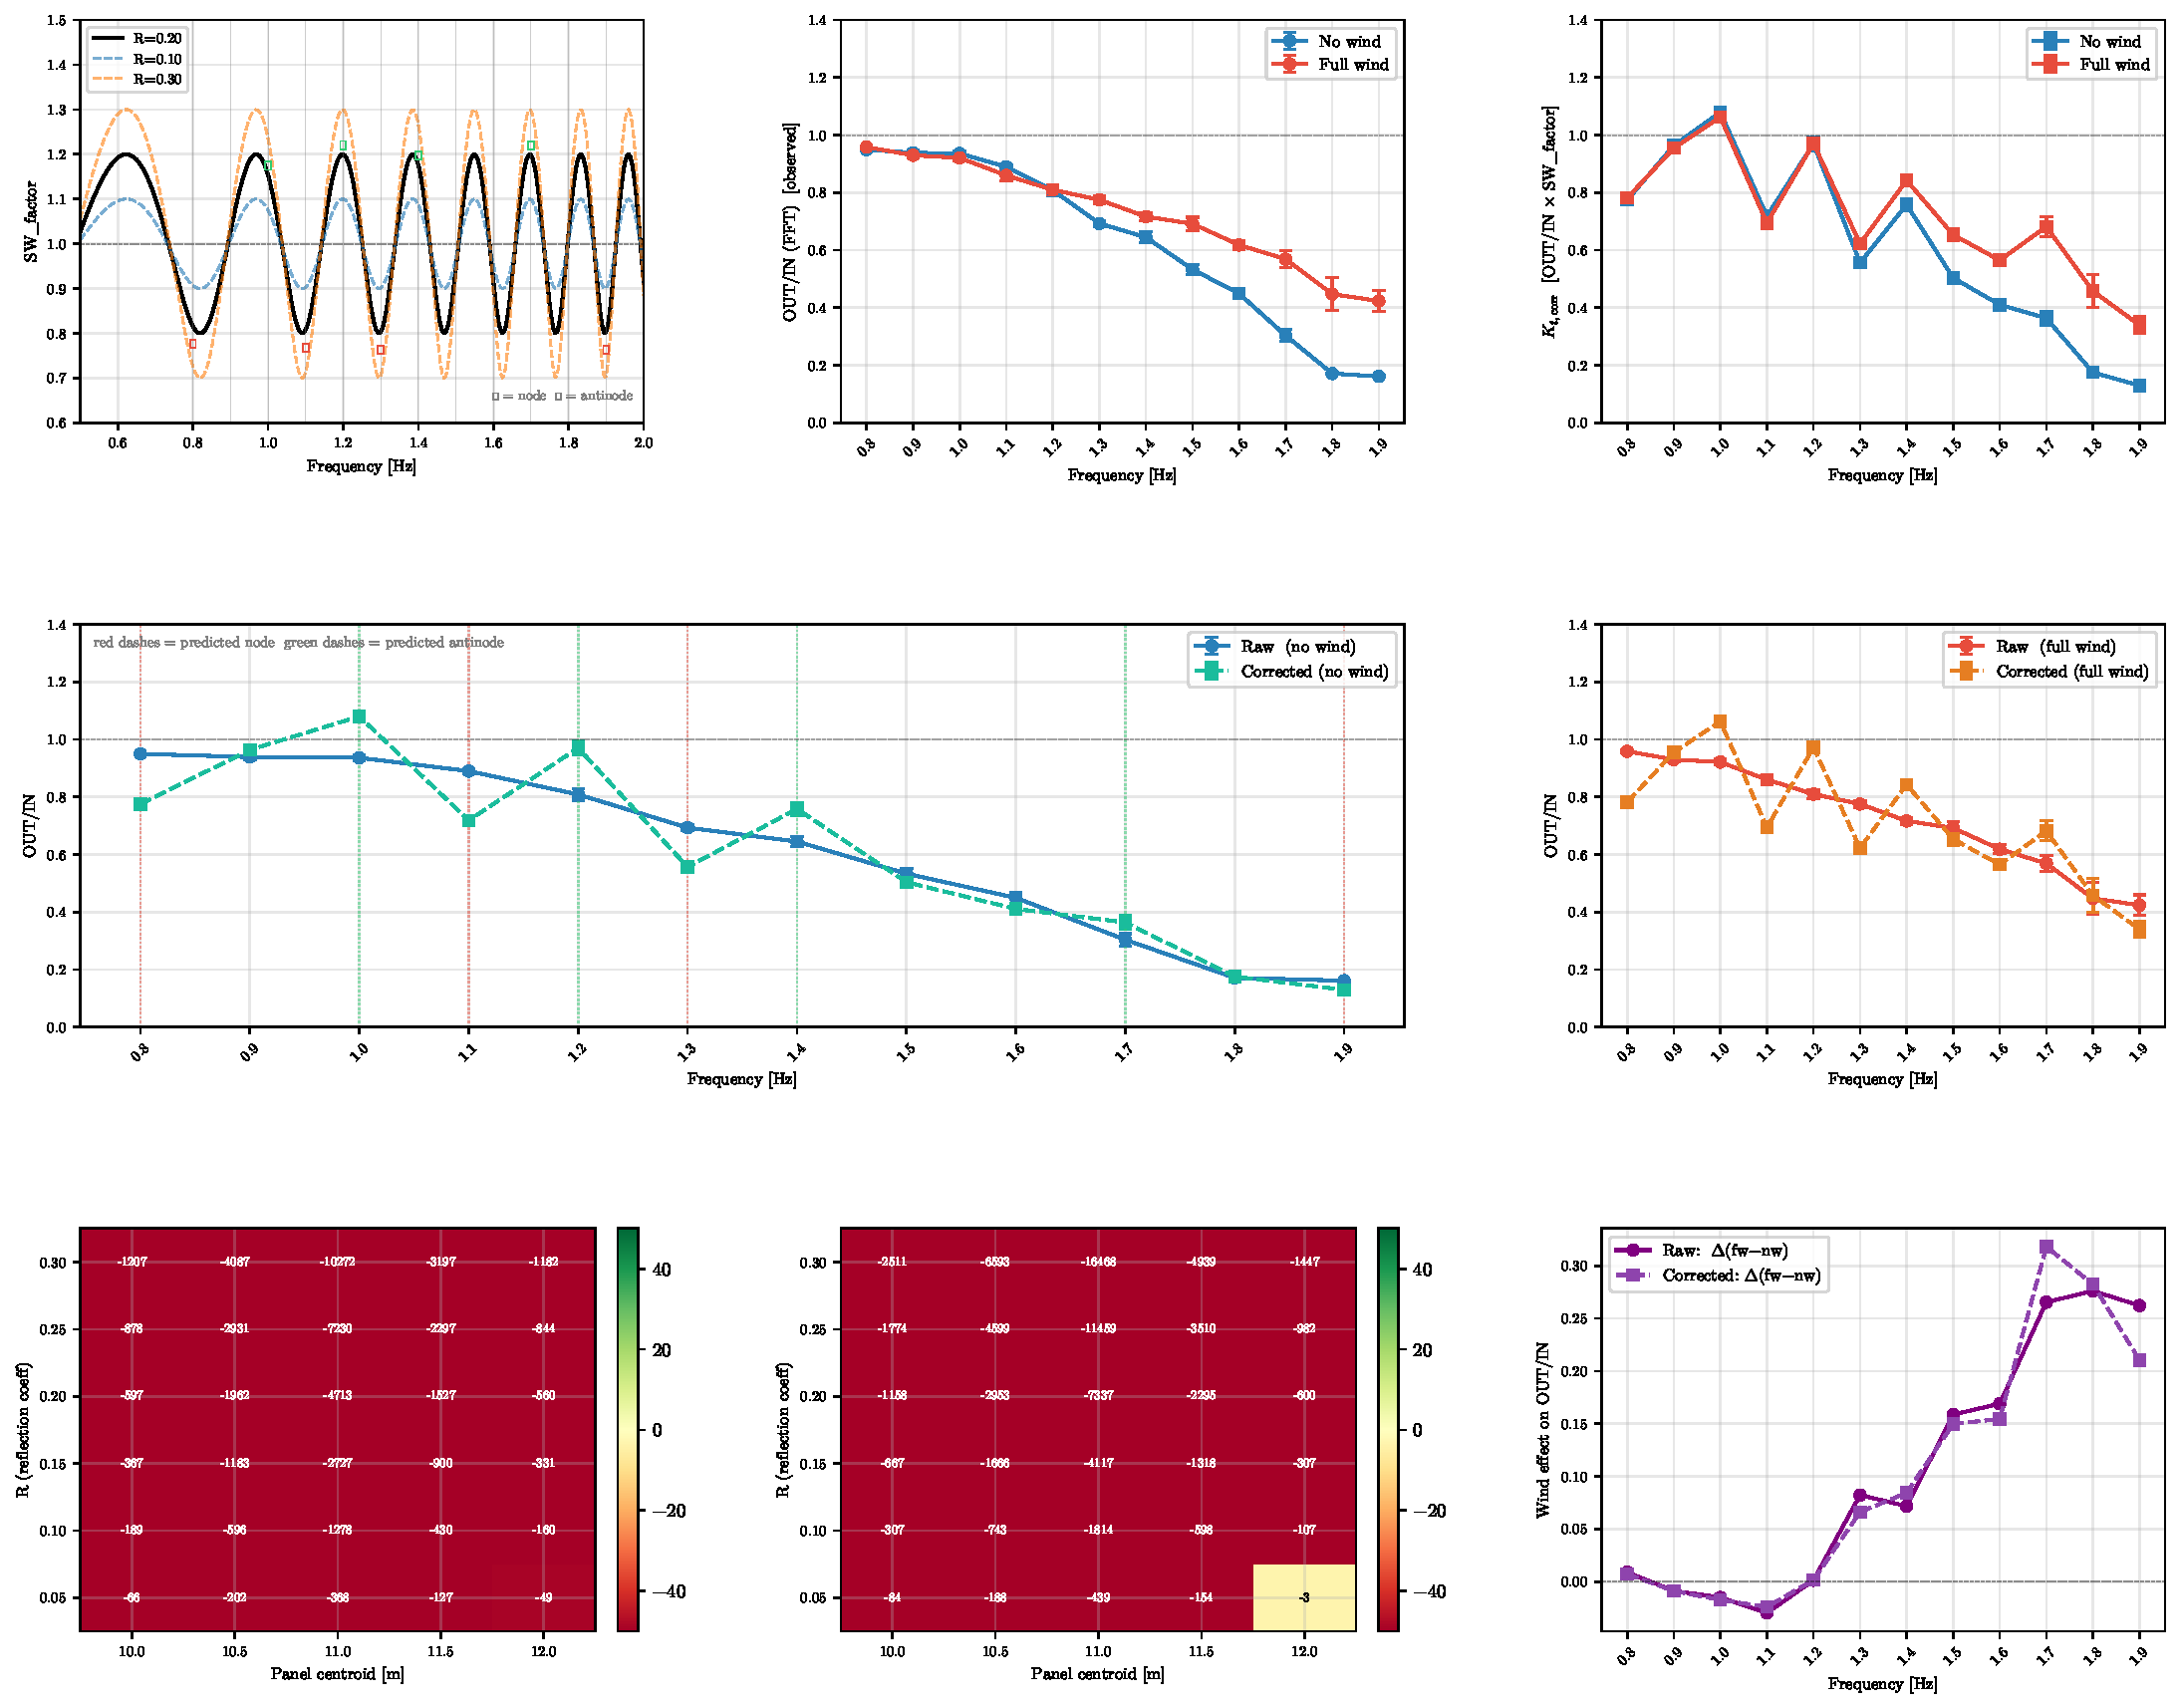
\includegraphics[width=0.95\linewidth]{FIGURES/ch04_sw_correction_test.pdf}
  \caption[Standing-wave correction test]{%
    Standing-wave correction test at R=0.20 on measured OUT/IN ratios. If the panel reflected a significant fraction of the incident wave, the OUT/IN(FFT) vs frequency curve would carry a node/antinode fingerprint with characteristic spacing $\Delta f = c_g/(4 x_\mathrm{{IN}})$. Applying a correction at R=0.20 to the raw OUT/IN curve creates a violent zigzag (top-right panel) — the raw data shows NO such pattern. This puts an upper bound of $R\lesssim0.05$ on the panel's reflection coefficient, consistent with the direct Mansard--Funke measurement (see CH04 \S4c). Conclusion: the raw OUT/IN(FFT) values require no standing-wave correction; the existing methodology is safe.
  }
  \label{fig:ch04_sw_correction_test}
\end{figure}
